\subsection{Storage Space and Impact on Fault Tolerance}
 
\begin{figure}
    \centering
    \subfigure[Sharing of data under VM-oblivious dedup model]
    {
        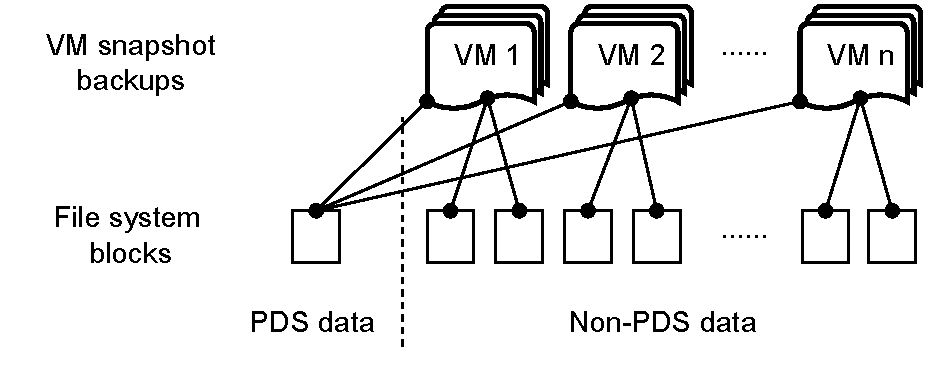
\includegraphics[width=3in]{images/share_vc.pdf}
        \label{fig:share_vc}
    }
    \\
    \subfigure[Sharing of data under VM-centric dedup model]
    {
        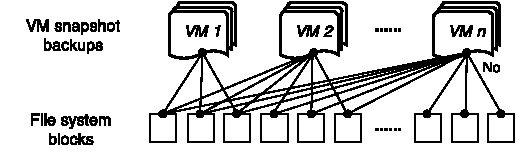
\includegraphics[width=3in]{images/share_vo.pdf}
        \label{fig:share_vo}
    }
    \caption{Difference of sharing data under VO and VC approaches}
    \label{fig:share}
\end{figure}

The replication degree of the backup storage 
is $r$ for regular file blocks and $r=3$ is a typical setting in the distributed
file system~\cite{Hadoop,GFS}.
In the VC approach, a special replica degree $r_c$ used for PDS blocks where $r_c>r$. 
Notice that the ratio of non-PDS data size vs PDS data size for each VM is
\[
\sigma=  \frac{c*\delta(1 -   (\frac{k}{c_u})^{1-\alpha})} {k}.
\]

Thus  storage cost for VO with full deduplication is $c_u *r$ and for VC, it is
\[ k*r_c  + k*\sigma *r.
\]

In our experiment with Alibaba data, the ratio $\sigma$ 
is 162. Thus allocation of extra replicas for PDS only introduces a small amount of extra space
cost.  Figure~\ref{fig:storageCDS} shows the storage cost ratio of VC and VO when 
$r$=3, and $r_c$ varies from 3 to 10.
The result shows that the storage cost for adding extra replication for PDS
is insignificant.


Next we  compare the impact of losing $d$ machines 
to the the VC and VO approaches.  


\comments{
For each rank $i$ block which appears $C_i$ times  among $V$ virtual machines.
Assigning this block to virtual machines can be viewed as a classical ball-bin assignment
approximated by a Poisson distribution. Namely the virtual machines that share this block
is approximated as $1 -  e^{C_i/V}$.
Thus the average number of VMs that share a block is:
\[
(1-\delta) + \delta \sum_1^{u_b} \frac{1 -  e^{C_i/V}}{u_b}.
\]
Any failure of a block would impact the above number of virtual machines.
In VO, the number of VMs that share a block is:
\[
\sum_1^{u_b'} \frac{1 -  e^{C_i'/V}}{u_b'}.
\]

Next we discuss how a failure of $d$ machines impacts the VM snapshots in VC.
When $d<r$, there is no loss of data in the snapshot storage.
When $r_c> d \ge r$, some of data blocks in the storage are lost, and we compute the number of VMs that could
suffer the loss of their snapshots.
When $d \ge r_c$, some of PDS blocks are affected.
In VC, the blocks in PDS are stored in a container manner (superblock), and they are shared by many VMs.
The number of data containers stored with replication degree $r$ for
referenced by each VM is:
\[
N_1= \frac{b}{v*s} (1-\delta) +b/(v*s)\delta (1 -  (\frac{k}{b_u})^{1-\alpha}).
\]
The number of PDS data containers stored with replication degree $r_c$ for
referenced by each VM is:
\[
N_2= \frac{b}{v*s}\delta (\frac{k}{b_u})^{1-\alpha}.
\]
}



%Thus the number of VMs using a block =    $(1-s_c)  + s_c *L$.
In characterizing the reliability of VM backups in our model, 
we consider the likely hood that a file system block fails,
given some number of storage machine failures. 
Every time a filesystem block fails,
we say that we have lost data for that virtual machine, so it is no longer
available. 
In reality it may be only one snapshot that is affected, but it is the user
who must decide which snapshots are important, so we consider the worst case. 
We use filesystem blocks rather than a deduplication
data chunk as our unit of failure because the DFS keeps
filesystem blocks as its base unit of storage.
% (in our case there are 
%16384 blocks in a filesytem block on average, with 4KB block size and 
%a 64MB block size).

To  compute the probablity of losing snapshots of a virtual machine, 
we estimate the number of file system blocks per VM in each apporach.
We can build a bipartite graph representing the association from unique file system blocks
to their corresponding VMs. An association edge is  drawn  from a file block  to a VM 
if this file is used by this VM. 
For VC, each VM has an 
averge number of $N_1$ file system blocks for non-PDS data. 
It also refers  an average of   $N_2$ file system blocks for PDS data 
For VO, each VM has an average  of  $N_o$ file system blocks
and let $V_o$ be the averge number of VMs shared by each file system block.
Figure~\ref{fig:shared} illustates the bipartite association.

In VC, each non-PDS file system block is associated with one VM while PDS file system blocks are
shared among VMs  (at most $V$ VMs). Thus, 
\[
V *N_1 *s  = pD  \frac{\delta} {\delta +1} \; \mbox{ and } \; 
V *N_2 *s  \leq pD  \frac{1} {\delta +1} *V.
\]
For the VO approach, 
\[
V *N_o *s  = pD  V_o.
\]
Then
\[
N_1= \frac{pD \delta} {V s (\delta +1)},\; 
N_2 \leq \frac{pD } {s (\delta +1)}, \; 
\mbox{and} \; N_o = \frac{pD V_o } {s V}.
\]
Since each file block (with default size $s=64MB$) contains many chunks (on average 4KB),
each file block contains the hot low-level chunks shared by many VMs, and it also contains
rare chunks which are not shared.
Figure~\ref{fig:VOshared} shows the number of VMs shared by each file block.
In our experiment, we find that $V_o \approx 0.2 V$ when backing up VMs one by one.
We can observe that $N_1 +N_2 << N_o$.
If  the backup for multiple VMs is conducted concurrently, there would be more
VMs shared  by each file block on average.

Figure~\ref{fig-fsb-links} shows the average number of VMs sharing a
filesystem block (FSB) in the global index as VMs are added. Two of the VMs had
much larger hard drives (\~300GB), which explains the 2 drops, as those two VMs
added much more unique data than normal. Though we expect the graph to level out some for
much larger datasets, it should continue to increase, which has important implications
on VM backup availability in the precense of failures. Below we show the
significant impact the number of links has on VM backup reliability.

\comments{%dropping block links bec. we don't use it elsewhere
\begin{figure}[ht]
  \centering
  %\includegraphics[scale=.45,natwidth=511,natheight=276]{vo_links}
	\begin{tikzpicture}
		\begin{axis}[
		%title={VO Block links},
		xlabel={Number of VMs added},
		ylabel={Avg. links to a chunk},
		%extra y ticks={4.5,5.5,6.5} %because it only shows 4,5,6,7
		legend pos=south east
		]
		\addplot[color=blue,mark=*] table[x=VMs,y=Measured] {figures/vo_links.txt};
		\addplot[color=red,mark=square*] table[x=VMs,y=Theoretical] {figures/vo_links.txt};
		\legend{Measured,Theoretical};
		\end{axis}
	\end{tikzpicture}
  \caption{Average number of VMs sharing a data chunk in the global index}
  \label{fig-vo-links}
\end{figure}
}

\begin{figure}[ht]
  \centering
	\begin{tikzpicture}
		\begin{axis}[
		%title={VO FSB links},
		xlabel={Number of VMs},
		ylabel={Avg. Num. VMs sharing FSB},
		%extra y ticks={4.5,5.5,6.5} %to show extra ticks
		legend pos=north west
		]
                \addplot[color=blue,mark=*] table[x=VMs,y=FSBLinks] {figures/vo_fsb_links.txt};
		\addplot[color=red,mark=square*] table[x=VMs,y=cdslinks] {figures/cds_links.txt};
                \legend{Global Dedup (VO), PDS FSB (VC)};
		\end{axis}
	\end{tikzpicture}
  \caption{Measured Average number of VMs sharing a 64MB FSB with global dedup (VO), and in a 2\% PDS for VC.}
  \label{fig-fsb-links}
\end{figure}

\begin{figure}[ht]
  \centering
	\begin{tikzpicture}
		\begin{axis}[
		%title={VO VM links},
		xlabel={Number of VMs},
		ylabel={Avg. Num. FSBs used by VM},
		%extra y ticks={4.5,5.5,6.5} %to show extra ticks
		legend pos=north west
		]
                \addplot[color=blue,mark=*] table[x=VMs,y=VMLinks] {figures/vo_vm_links.txt};
		\addplot[color=red,mark=square*] table[x=VMs,y=VMNonCDSLinks] {figures/vc_vm_links.txt};
		\addplot[color=red,densely dashed,mark=triangle*,mark size=3] table[x=VMs,y=VMCDSLinks] {figures/vc_vm_links.txt};
                \legend{VO FSB, Non-PDS FSB (VC), PDS FSB (VC)};
		\end{axis}
	\end{tikzpicture}
  \caption{Measured Average number of 64MB FSBs used by a single VM. For VC both the number of PDS and Non-PDS FSBs used are shown.}
  \label{fig-vm-links}
\end{figure}

The snapshot availability of is a VM is the likelyhood that
there is no  data loss for all its file blocks.
With replication degree $r$, the likelyhood of
a file block block is the probability that  
all of its replicas appear in $d$ failed machines. 
Namely, $\binom{d}{r}/ \binom{p}{r}$.


When there are $r \le d<r_c$ machines failed and then there is no PDS data loss,  
%a file block failure depends on if all replicas of this container reside in the failed machines.
the snapshot avaiability of a VM in the VC approach is 
and is
\[
(1-\frac{\binom{d}{r}} { \binom{p}{r} })^{N_1}.
\]
%\begin{multline}
%= Probability (\mbox{ There is no file block loss in this VM}) \\
%= Probability(\mbox{ A file block has file data loss})^{N_1}\\
%= (1- Probability (\mbox{all replicas of its block fail}))^{N_1}\\
%\end{multline}
%\end{split}

When $r_c \leq d$, both non-PDS and PDS file blocks in VC can have a loss.
The snapshot availability of  a VM in the VC approach is
\[
(1-\frac{ \binom{d}{r}} { \binom{p}{r} })^{N_1} 
*
(1-\frac{ \binom{d}{r_c}} { \binom{p}{r_c} })^{N_2}.
\]
%= Probability(\mbox{ No non-PDS file block loss})^{N_1}
%Probability(\mbox{ No PDS file block loss})^{N_2}\\
%\begin{multline}
%\end{split}
%\end{multline}

The snapshot availability of a VM  in the VO approach is
\[ 
(1-\frac{ \binom{d}{r}} { \binom{p}{r} })^{N_o}. 
\]



%By comparison, the probability that a VM has data loss is close to
%1 once  there are  $d \ge r$ failed machines. That is because there are more data blocks
%shared among VMs. Any failure of these blocks causes many more VMs to fail.

%%%%%%%%%%%%%%%%%%%%%%%%%%%%%%%%%%%%OLD MODEL START%%%%%%%%%%%%%%%%%%%%%%%%%%%%%%%%%%%%%%%%%%%%%%%%%%%%%%%%%%%%%%%
%The rate of increase in node failures can be seen in Figure~\ref{fig-vm-failure}
%(for a 100 node cluster).
%The graph assumes 10X40GB snapshots per VM with 18\% unique data after local
%dedup and 64MB filesytem chunks (which results in 1792 filesystem chunks per
%VM). We assume 18\% unique data after local dedup because that is what our
%snapshots have shown.

\comments{\begin{figure}[ht]
  \centering
  %\includegraphics[scale=.45,natwidth=511,natheight=276]{vo_links}
	\begin{tikzpicture}
		\begin{axis}[
		%title={Node failure affect on VMs},
		xlabel={Number of nodes failed},
		ylabel={chance that a VM is affected (\%) in VO},
		%extra y ticks={4.5,5.5,6.5} %because it only shows 4,5,6,7
		]
		\addplot[color=blue,mark=*] table{figures/vm_failure.txt};
		\end{axis}
	\end{tikzpicture}
  \caption{Percent chance that a VM is affected as storage nodes fail}
  \label{fig-vm-failure}
\end{figure}}

\comments{\begin{figure}[ht]
  \centering
  %\includegraphics[scale=.45,natwidth=511,natheight=276]{vo_links}
	\begin{tikzpicture}
		\begin{axis}[
		%title={Node failure affect on VMs},
		xlabel={Failed storage nodes},
		ylabel={Chance VM is affected (\%)},
		%extra y ticks={4.5,5.5,6.5} %if important numbers are missing
                mark options=solid,
                legend pos=north west
		]
                \addplot[densely dashed,color=blue,mark=*] table[x=NodesFailed,y=VO]{figures/vm_failure_1.txt};
                \addplot[color=red,mark=*] table[x=NodesFailed,y=VC1]{figures/vm_failure_1.txt};
                \addplot[color=red,mark=square*] table[x=NodesFailed,y=VC2]{figures/vm_failure_1.txt};
                \addplot[color=red,mark=triangle*,mark size=3] table[x=NodesFailed,y=VC3]{figures/vm_failure_1.txt};
                \legend{$VO$,$VC_{C_R=3}$,$VC_{C_R=4}$,$VC_{C_R=5}$,$VC_{C_R=6}$,$VC_{C_R=7}$}
		\end{axis}
	\end{tikzpicture}
  \caption{Percent chance that a VM is affected as storage nodes fail}
  \label{fig-vm-failure}
\end{figure}}

%%%%%%%%%%%%%%%%%%%%%%%%%%%%%%%%%%%%%%%%%OLD MODEL END%%%%%%%%%%%%%%%%%%%%%%%%%%%%%%%%%%%%%%%%%%%%%%%%%%%%%%%%%%%%%%

%%%%%%%%%%%%%%%%%%%%%%%%%%%%%%%%%%%%%%%%%NEW MODEL START%%%%%%%%%%%%%%%%%%%%%%%%%%%%%%%%%%%%%%%%%%%%%%%%%%%%%%%%%%%%


\comments{
We take the likelyhood of VM failure to be the same as the likelyhood of chunk failure,
so
\[
    P_{VMfailure}=\frac{\binom{d}{r}}{\binom{p}{r}}
\]

Since both in the PDS and in the VO approach a single filesystem chunk may be used by many VMs,
we must multiply the block failure ratio by the number of outgoing links for the block to get
the expected impact on the system.
\[
    E_{VMfailure}=L\frac{\binom{d}{r}}{\binom{p}{r}}
\]

in our current testbed we have measured the average number of links per chunk
(Figure~\ref{vo-links}) and number of links per Filesystem Block (FSB)
(Figure~\ref{fig-fsb-links}) in our dataset. For the complete dataset, we also
found the average number of links to PDS chunks, which was \~19 using a 2\%
PDS. From Figure~\ref{fig-fsb-links} you can see that as you add VMs, the
average number of links to a chunk increases linearly for our dataset. We
expect that this trend will level out with larger datasets, but should continue
to increase at a slower rate.  For the VC model, we have to consider both PDS
chunks and non-PDS chunks. In the VO model all data is shared, but in VC only
the PDS data is shared, but at a much higher rate. This gives a strong
advantage to VC, in that for a large percent of the data (95-99\%), there is
only one VM pointing to each non-PDS chunk. You can see the increase in
reliability in Figure~\ref{fig-vm-availability}.
}

Figure~\ref{fig-vm-availability} shows the reliability of VM backups as storage
nodes fail for different numbers of links to average blocks in the index. We
chose 5 and 20 for the VO and VC block links counts because those are what we
measured in our dataset, and chose higher numbers to account for much larger
datasets. We chose to use a very optimistic setting for VO (10), and an extreme
amount of sharing for VC (1000) to better show the significant improvement in
data reliability for the VC model (showing VO best case is still worse than VC
worst case). As you can see from the graph, even small changes in the number of
links to VO blocks has a significant impact on reliability, while even a 50
times increase in the VC block link counts only slightly affects VC
reliability.  The key factor placed is that  $N_1 +N_2 << N_o$, caused by the
fact that the VM-centric approach localizes deduplication and packs  data
blocks for one VM as much as possible.  The extra replicaton for PDS blocks
also signficantly increases the snapshot availability even when a PDS file
block is shared by every VM.

% while in VO even small increases in $L$ causes a large decrease in availability. 
Figure~\ref{fig-pds-replication}
shows the advantages of increasing the replication factor for PDS blocks. the
numbers in the graph are only meant to be relative, as we assume higher PDS
block links than we have measured in our dataset (to account for a much larger
body of data). It is easy to see though that increasing the replication of just
the PDS blocks (which are the most popular blocks) can have a positive impact
on the overall reliablity of the VM backups. These figures together show the
advantages of the VM-centric model, and the advantages that separating the
replication factor for popular blocks can have on reliability.

\begin{table}
    \begin{tabular}{|l|ll|}
    \hline
    \multirow{2}{*}{Nodes Failed}   & \multicolumn{2}{c|}{Availability(\%)}\\
                                    & $R=3$ & $R=4$\\
    \hline
    1           &  100      & 100\\
    2           & 100       & 100\\
    3          & 99.999     & 100\\
    5          & 99.993     & 99.9999\\
    10          & 99.926    & 99.995\\
    20          & 99.295    & 99.876\\
    \hline
    \end{tabular}
    \caption{Availability of a single FSB in the global data store with different relplication factors}
    \label{tab:fsb-availability}
\end{table}

\begin{figure}[ht]
  \centering
    \begin{tikzpicture}
            \begin{axis}[
            %title={FSB Availability},
            xlabel={Number of Machines Failed},
            ylabel={Availability of Single FSB (\%)},
            %extra y ticks={4.5,5.5,6.5} %to add extra ticks
            mark options=solid,
            legend pos=south west,
            %legend columns=2,
            %legend style={
            %    at={(0.5,-0.2)},
            %anchor=north}
            ]
            \addplot[color=blue,mark=none] table[x=NodesFailed,y=Availability3] {figures/fsb_availability.txt};
            \addplot[densely dashed, color=red,mark=none] table[x=NodesFailed,y=Availability4] {figures/fsb_availability.txt};
            \legend{$R=3$,$R=4$};
            \end{axis}
    \end{tikzpicture}
    \caption{Availability of Individual FSBs in 100 Machine Cluster with different replication factors.}
  \label{fig-fsb-availability}
\end{figure}


\begin{figure}[ht]
  \centering
  %\includegraphics[scale=.45,natwidth=511,natheight=276]{vo_links}
	\begin{tikzpicture}
		\begin{axis}[
		%title={Node failure affect on VMs},
		xlabel={Failed storage nodes},
		ylabel={VM Snapshot Availability (\%)},
		extra y ticks={99.9}, %if important numbers are missing
                mark options=solid,
                legend style={
                    cells={anchor=west}, %legend entry alignment
                    legend pos=south west %legend position
                }
		]
                \addplot[densely dashed,color=blue,mark=square*] table[x=NodesFailed,y=VO2]{figures/vm_failure_2.txt};
                \addplot[densely dashed,color=blue,mark=*] table[x=NodesFailed,y=VO1]{figures/vm_failure_2.txt};
                %\addplot[densely dashed,color=blue,mark=triangle*,mark size=3] table[x=NodesFailed,y=VO3]{figures/vm_failure_2.txt};
                %\addplot[densely dashed,color=blue,mark=diamond*,mark size=3] table[x=NodesFailed,y=VO4]{figures/vm_failure_2.txt};
                \addplot[color=red,mark=square*] table[x=NodesFailed,y=VC2]{figures/vm_failure_2.txt};
                \addplot[color=red,mark=*] table[x=NodesFailed,y=VC1]{figures/vm_failure_2.txt};
                %\addplot[color=red,mark=triangle*,mark size=3] table[x=NodesFailed,y=VC3]{figures/vm_failure_2.txt};
                %\addplot[color=red,mark=diamond*,mark size=3] table[x=NodesFailed,y=VC4]{figures/vm_failure_2.txt};
            \legend{$VO\,10$ (optimistic),$VO\,5$ (measured),$VC\,1000$ (extreme),$VC\,20$ (measured)}
		\end{axis}
	\end{tikzpicture}
  \caption{Availability of VM backups as nodes fail for VO and VC models for varying degrees of block sharing (i.e. average number of VMs that use a block). Non-PDS replication fixed at 3 and PDS replication increased to 4.}
  \label{fig-vm-availability}
\end{figure}

\begin{figure}[ht]
  \centering
	\begin{tikzpicture}
		\begin{axis}[
		%title={PDS Replication affect on availability},
		xlabel={Failed storage nodes},
		ylabel={VM Snapshot Availability (\%)},
		extra y ticks={99.9}, %if important numbers are missing
                mark options=solid,
                legend style={
                    cells={anchor=west}, %legend entry alignment
                    legend pos=south west %legend position
                }
		]
                \addplot[color=blue,mark=*] table[x=NodesFailed,y=VC1]{figures/cds_replication.txt};
                \addplot[color=red,mark=square*] table[x=NodesFailed,y=VC2]{figures/cds_replication.txt};
                \addplot[color=brown,mark=triangle*,mark size=3] table[x=NodesFailed,y=VC3]{figures/cds_replication.txt};
                \addplot[color=black,mark=diamond*,mark size=3] table[x=NodesFailed,y=VC4]{figures/cds_replication.txt};
            \legend{$R_C=3$,$R_C=4$,$R_C=5$,$R_C=7$}
		\end{axis}
	\end{tikzpicture}
  \caption{Availability of VM backups as nodes fail in the VC model for different PDS Replication factors (Non-PDS replication fixed at 3, and average PDS block links set to 1000)}
  \label{fig-pds-replication}
\end{figure}


%%%%%%%%%%%%%%%%%%%%%%%%%%%%%%%%%%%%%%%%NEW MODEL END%%%%%%%%%%%%%%%%%%%%%%%%%%%%%%%%%%%%%%%%%%%%%%%%%%%%%%%%%%%%%%

\comments{
We use the following parameters  during the analysis
\begin{itemize}
\item 	$V$ is the number of VMs. $m$ is the number of physical machines hosting the backup storage.
$d$ is the number of machines failed.
\item In the VC approach, $s_c$  of them in the backup storage
are shared by others with a zipf distribution. $(1-s_c)$ 
of them  is unique (nobody shares with them).
$L_c$ is the average number of VMs sharing a block (if it is in PDS for the VC approach.
$b_c$ is the number of shared blocks in VC.
\item In the VO approach, $s_o$ is the number of blocks shared.
$L_o$ is the average number of VMs sharing a block. 
\item $b$ is the  number of blocks stored in the storage after deduplication.
 \end{itemize}

The distribution of data blocks shared among VMs in VC follows a zipf distribution.
Given a VM block, the probability of being rank $x$ block is $P(x) = P(1) * x^{-\alpha}$
where $P(1)$ is the probability of being rank 1 most popular block.
Since $\sum P(x)= 1$, $P(1)= \frac{1}{\sum_1^{b_c} x^{-\alpha} }$.
Let $y$ be the number of VMs sharing rank $x$ block in VC, and  then  $y= V* P(x)$.

Thus the average number of VMs sharing a data block in the VC backup storage is:
\begin{equation}
%\begin{align}
\begin{split}
L_c& =  (1-s_c)*1 + s_c \sum_1^{b_c} P(x) * y \\
& =  (1-s_c)*1 + s_c \sum P(1)^2 *  x^{-2\alpha} *  V.
\end{split}
%\end{align}
\end{equation}



Under $d$ failed machines, the  expected number of VMs 
which suffer from data loss in VC is
\begin{multline}
%\begin{split}
 \sum_{1}^{V}  ( Probability (\mbox{ a VM fails)}) \\
= \sum_{1}^{V}  ( 1- Probability (\mbox{ a VM has no data loss)}) \\
= V ( 1-  Probability(\mbox{ A block has no data loss} )^{L_c} ).
%\end{split}
\end{multline}

%Thus the number of VMs using a block =    $(1-s_c)  + s_c *L$.

When there are $d$ machines failed and the probability of
a block failure depends on if all replicas of this block reside in the failed machines.
When $r< d <r_c$,  only unshared data blocks can fail in VC. Then
%Probablity(\mbox { no loss for this  block}) = 1 - Probability (\mbox{ this block in d failed machiens})
\begin{multline}
%\begin{split}
Probability(\mbox{ A block has data loss})\\
= (1-s_c) (1- Probability (\mbox{ this block in d failed machines}))\\
= (1-s_c) (1- \frac{ \binom{d}{r}} { \binom{m}{r} }).
%\end{split}
\end{multline}
When $r_c \leq d$, shared data blocks in VC can have a loss. 
\[
Probability(\mbox{A block has data loss})
= 
(1-s_c) (1- \frac{ \binom{d}{r}} { \binom{m}{r} })
+ s_c (1- \frac{ \binom{r_c}{d}} { \binom{m}{r_c} }).
\]

By comparison, under $d$ failed machines, the  expected number of VMs 
which suffer from data loss in VO is
\[
V ( 1-  (1- \frac{ \binom{d}{r}} { \binom{m}{r} })^{L_o} ).
\]
where
\[
L_o = (1-s_o) + s_o \sum_1^b  P(1)^2 *  (x')^{-2\alpha'} *V.  
\]

%the above model assumes uniform distribution of blocks and doesn't provide compelling numbers
%with 3 replicas, 100 machines, and only 3 failures the chance of a single 10GB VM surviving is 9.11*10^-8
%if we wanted to include it we probably want a model that includes containers, but that might be too complex
%to be useful.
}


\comments{
	=  sum _for_all_block(   Probablity (a block fails) *number of VM sharing this block ))
               = Probability(a block fails) * sum_for_all_blocks (numb of VM shared)
	= Probablity (a block fails) *b *aveageLengthVM
	= [ 1-  C(r, k) /C(n,r)] * b* [ 1+ s *V(1-1/ln V)]
  
----------------------------------------------------------------------       

\subsection{Empirical Validation}
%To validate our theoritical model for the probability of data loss, we computed
%the number of snapshots using each block in a global index for the 350 snapshot
%traces. As you can see in Fig.~\ref{??}, The average number of VMs sharing a block
%%TODO: insert figure generated from data/links_no_cds.dat
%increases linearly with the number of snapshots. For 350 snapshots there are an
%average of 13.1 links to a given block in the global index.
To validate our theoretical model for the probability of data loss, we measured
the number of snapshots and VMs sharing data blocks for our 350 snapshot
dataset. As you can see in Fig.~\ref{??}, the average number of snapshots sharing
a block increases linearly with the number of snapshots. For 350 snapshots
there are an average of 13.1 incoming links to a given data block in the global
index. If we look at the number of VMs sharing a data block rather than
snapshots, in the full dataset on average 1.47 VMs point to a data block in the
index.
%What else do we need from the simulation to validate the model?

\subsubsection{PDS and Fault Tolerance}
%all numbers in this paragraph need to be corrected after I re-run the tests
%using the actual cds generator code
As part of our emprirical validation of our model, we also computed the effects
of the PDS on fault tolerance. If we exclude the top 5\% most popular blocks
and set aside those in the PDS, the average number of links to a non-PDS block
%TODO: insert figure generated from data/links_cds.dat and data/links_wo_cds.dat
drops to 10.3 for 350 snapshots. This means that on average, \~3 fewer
snapshots will be affected by a lost data block in the general data store.
The average number of links to a PDS block however, for 350 snapshots, is
65.7. This suggests that a much higher replication factor is warranted for
the PDS, as on average, a PDS block appears in \~20\% of all the snapshots.
These measured numbers are different from our theoritical model due to the fact
that duplicate data blocks are not uniformly distributed across all VMs.
With uniform distribution of duplicates (and a zipf distribution on the number
of duplicates), there should be on average 2.55 incoming VM links to each
block. Since we show the average number of links to be 1.47 in our actual
traces, the duplicates are
more tighly grouped than the uniform model would predict. This supports
the benefits of using a PDS plus more localized deduplication.

The PDS gives a clear boundary for setting different replication factors,
And our tests suggest that by separating the replication factor for the PDS
and non-PDS blocks, greater fault tolerance can be acheived.

----------------------------------------------------------------------

For PDS model, 85\% blocks are using the data from the same VM while upto 10\% data is for PDS (we actually only use 5% perhaps).  Thus the overall speaking, at most 10% of data are shared.
Thus  for PDS approach,   the # VM failure caused by k machines is at most  [ 1-  C(r, k) /C(n,r)] * b* [ 1+ 0.10 *V(1-1/ln V)].
For original approach,  [ 1-  C(r, k) /C(n,r)] * b* [ 1+ 0.90 *V(1-1/ln V)].
For large V, the reliability improves by 9 times.
}
